%==============================================================================
% APRESENTAÇÃO BEAMER - VERSÃO FINAL COM PGFPLOTS REINTEGRADO
%==============================================================================

\documentclass{beamer}

%==============================================================================
% 1. TEMA E ESTRUTURA VISUAL
%==============================================================================
\usetheme{metropolis}

%==============================================================================
% 2. PACOTES ESSENCIAIS
%==============================================================================
\usepackage{tikz}
\usepackage{pgfplots}
\usepackage{pgfplotstable}
% Definimos a compatibilidade para garantir o funcionamento correto das funcionalidades
\pgfplotsset{compat=1.18}
\usepackage{booktabs} % Para tabelas com melhor formatação

%==============================================================================
% 3. CONFIGURAÇÃO DE FONTES
%==============================================================================
\usepackage[light]{sourcesanspro}

%==============================================================================
% 4. PALETA DE CORES E IDENTIDADE VISUAL
%==============================================================================
\definecolor{crpPrincipal}{HTML}{422C73}
\definecolor{crpSecundaria2}{HTML}{BF73AB}

\setbeamercolor{normal text}{fg=crpPrincipal, bg=white}
\setbeamercolor{progress bar}{fg=crpSecundaria2, bg=crpPrincipal!20}
\setbeamercolor{frametitle}{bg=crpPrincipal, fg=white}
\setbeamercolor{alerted text}{fg=crpSecundaria2}
\setbeamercolor{subtitle}{fg=crpPrincipal}

%==============================================================================
% 5. DEFINIÇÃO E CARREGAMENTO DOS DADOS (PARA PGFPLOTS)
%==============================================================================
% Dados reorganizados por ano para barras empilhadas
\pgfplotstableread[col sep=comma, header=true]{%
	ano, cadernos, cartilhas, livros, revista, orienta, manuais
	2006, 0, 0, 1, 0, 0, 1
	2007, 5, 0, 0, 0, 0, 1
	2008, 1, 0, 0, 0, 0, 1
	2009, 1, 0, 0, 0, 0, 0
	2010, 3, 2, 2, 0, 0, 1
	2011, 3, 0, 0, 0, 0, 0
	2012, 1, 0, 0, 0, 0, 0
	2013, 0, 0, 2, 0, 0, 1
	2014, 0, 3, 1, 0, 0, 1
	2015, 2, 1, 0, 0, 0, 0
	2016, 6, 1, 8, 0, 0, 1
	2017, 0, 0, 2, 0, 0, 0
	2018, 0, 0, 0, 0, 0, 0
	2019, 16, 2, 9, 0, 0, 1
	2020, 1, 0, 0, 0, 0, 1
	2021, 0, 0, 0, 0, 0, 2
	2022, 2, 0, 1, 0, 0, 0
	2023, 0, 0, 0, 0, 0, 2
	2024, 0, 0, 0, 0, 22, 0
	2025, 0, 3, 0, 1, 0, 1
}\publicacoesGeral

\pgfplotstableread[col sep=comma, header=true]{%
	ano, volumes
	2025, 2
	2024, 4
	2023, 2
	2022, 3
	2021, 1
	2020, 1
	2019, 4
	2018, 3
	2017, 1
	2016, 5
	2015, 5
	2014, 5
	2013, 5
	2012, 2
	2011, 3
	2010, 6
	2009, 6
	2008, 3
	2007, 6
	2006, 5
	2005, 4
	2004, 4
	2003, 4
	2002, 5
	2001, 6
	2000, 5
	1999, 6
	1998, 6
	1997, 7
	1996, 7
	1995, 7
	1994, 7
	1993, 5
	1992, 6
	1991, 7
	1990, 6
	1989, 7
	1988, 8
	1987, 3
	1986, 8
	1985, 8
	1984, 13
	1983, 9
	1982, 6
	1981, 7
}\publicacoesJornal

%==============================================================================
% 6. METADADOS DO DOCUMENTO
%==============================================================================
\title{Publicações impressas e digitais}
\subtitle{\textcolor{crpPrincipal}{Livros, cartilhas, Jornal Psi}}
\author{Conselho Regional de Psicologia de São Paulo}
\date{Outubro de 2025}

%==============================================================================
% INÍCIO DO DOCUMENTO
%==============================================================================
\begin{document}

	\begin{frame}[plain]
		\titlepage
	\end{frame}

\part{Publicações}
	\section{Histórico}
	\begin{frame}[fragile]{Linhas editoriais (categorias no site)}
		\begin{tikzpicture}
			\begin{axis}[
				width=0.85\textwidth, height=0.65\textheight,
				title={Distribuição anual das publicações por categoria (2006–2025)},
				xlabel={ano de publicação},
				ylabel={volumes publicados},
				font=\sffamily\small,
				title style={font=\sffamily\bfseries},
				label style={font=\sffamily\scriptsize},
				tick label style={font=\sffamily\tiny},
				xticklabel style={rotate=45, anchor=east, /pgf/number format/.cd, set thousands separator={}},
				xmin=2005.5, xmax=2025.5,
				ymin=0,
				xtick=data,
				ybar stacked,
				bar width=8pt,
				axis line style={thin},
				grid=major,
				grid style={thin, dashed, color=crpPrincipal!20},
				legend style={
					at={(0.5,-0.2)},
					anchor=north,
					legend columns=2,
					font=\sffamily\tiny,
					draw=none,
					/tikz/every even column/.append style={column sep=0.5cm}
				},
				]

				% Cada categoria é uma série empilhada
				\addplot[fill=crpPrincipal, draw=none]
					table [x=ano, y=cadernos] {\publicacoesGeral};
				\addlegendentry{Cadernos Temáticos}

				\addplot[fill=crpSecundaria2, draw=none]
					table [x=ano, y=cartilhas] {\publicacoesGeral};
				\addlegendentry{Cartilhas}

				\addplot[fill=crpSecundaria2!60, draw=none]
					table [x=ano, y=orienta] {\publicacoesGeral};
				\addlegendentry{CRP SP Orienta}

				\addplot[fill=crpPrincipal!60, draw=none]
					table [x=ano, y=livros] {\publicacoesGeral};
				\addlegendentry{Livros}

				\addplot[fill=crpPrincipal!40, draw=none]
					table [x=ano, y=manuais] {\publicacoesGeral};
				\addlegendentry{Manuais}

				\addplot[fill=crpSecundaria2!40, draw=none]
					table [x=ano, y=revista] {\publicacoesGeral};
				\addlegendentry{Rev. Práticas Psi}

			\end{axis}
		\end{tikzpicture}
	\end{frame}

\begin{frame}[fragile]{Publicações: visualizações e engajamento}
	\begin{columns}[T]
		\begin{column}{0.32\textwidth}
			\centering
			{\tiny\textbf{Usuários ativos}}
			\begin{tikzpicture}
				\begin{axis}[
					width=\textwidth,
					height=0.5\textheight,
					ybar,
					bar width=20pt,
					ymin=0,
					ymax=900,
					ylabel={milhares},
					ylabel style={font=\tiny},
					symbolic x coords={Site, Publicações},
					xtick=data,
					xticklabel style={font=\tiny, rotate=45, anchor=east},
					ytick style={font=\tiny},
					yticklabel style={font=\tiny},
					nodes near coords,
					nodes near coords style={font=\tiny, anchor=south},
					enlarge x limits=0.5,
					axis line style={thin},
					grid=major,
					grid style={thin, dashed, color=crpPrincipal!20},
					/pgf/number format/.cd,
					use comma,
					1000 sep={.},
					]
					\addplot[fill=crpPrincipal, draw=none]
						coordinates {(Site, 740) (Publicações, 49.4)};
				\end{axis}
			\end{tikzpicture}
		\end{column}

		\begin{column}{0.32\textwidth}
			\centering
			{\tiny\textbf{Visualizações}}
			\begin{tikzpicture}
				\begin{axis}[
					width=\textwidth,
					height=0.5\textheight,
					ybar,
					bar width=20pt,
					ymin=0,
					ymax=6.5,
					ylabel={milhões},
					ylabel style={font=\tiny},
					symbolic x coords={Site, Publicações},
					xtick=data,
					xticklabel style={font=\tiny, rotate=45, anchor=east},
					ytick style={font=\tiny},
					yticklabel style={font=\tiny},
					nodes near coords,
					nodes near coords style={font=\tiny, anchor=south},
					enlarge x limits=0.5,
					axis line style={thin},
					grid=major,
					grid style={thin, dashed, color=crpPrincipal!20},
					/pgf/number format/.cd,
					use comma,
					1000 sep={.},
					]
					\addplot[fill=crpPrincipal, draw=none]
						coordinates {(Site, 5.5) (Publicações, 0.094)};
				\end{axis}
			\end{tikzpicture}
		\end{column}

		\begin{column}{0.32\textwidth}
			\centering
			{\tiny\textbf{Tempo de engajamento}}
			\begin{tikzpicture}
				\begin{axis}[
					width=\textwidth,
					height=0.5\textheight,
					ybar,
					bar width=20pt,
					ymin=0,
					ymax=1900,
					ylabel={segundos},
					ylabel style={font=\tiny},
					symbolic x coords={Site, Publicações},
					xtick=data,
					xticklabel style={font=\tiny, rotate=45, anchor=east},
					ytick style={font=\tiny},
					yticklabel style={font=\tiny},
					nodes near coords,
					nodes near coords style={font=\tiny, anchor=south},
					enlarge x limits=0.5,
					axis line style={thin},
					grid=major,
					grid style={thin, dashed, color=crpPrincipal!20},
					/pgf/number format/.cd,
					use comma,
					1000 sep={.},
					]
					\addplot[fill=crpPrincipal, draw=none]
						coordinates {(Site, 1597.22) (Publicações, 52.84)};
				\end{axis}
			\end{tikzpicture}
		\end{column}
	\end{columns}

	\vspace{0.3cm}
	{\tiny
	\textbf{Insights:} A seção "Publicações" representa \alert{6,7\%} dos usuários, \alert{1,7\%} das visualizações e tem \alert{30x menos engajamento}.
	Confirma-se o perfil de \alert{consulta rápida} de documentos específicos.
	}
\end{frame}


%------------------------------------------------------------------------------
% SLIDE 4: TOP 15 PÁGINAS DA SEÇÃO /IMPRESSO/ (CORRIGIDO)
%------------------------------------------------------------------------------
\begin{frame}{15 páginas de publicação mais acessadas no site}
	\centering
	{\tiny
	\begin{tabular}{lrrrr}
		\toprule
		\textbf{Página} & \textbf{Visual.} & \textbf{Porc.} & \textbf{Usuários} & \textbf{Engaj.} \\
		\midrule
		\textbf{Índice de publicações} & \textbf{67.713} & \textbf{71,8\%} & \textbf{27.944} & \textbf{81,2} \\
		\midrule
		Manual de Prontuários & 2.730 & 2,9\% & 2.087 & 12,7 \\
		Jornal Psi n. 207 & 751 & 0,8\% & 604 & 14,5 \\
		Guia Acessibilidade & 627 & 0,7\% & 490 & 11,7 \\
		Atuação em Consultório & 555 & 0,6\% & 491 & 14,6 \\
		CT 15 Direitos Humanos & 533 & 0,6\% & 451 & 15,4 \\
		Manual de Orientações 2014 & 518 & 0,5\% & 405 & 15,1 \\
		Jornal Psi n. 206 & 491 & 0,5\% & 405 & 17,3 \\
		CIP definitiva & 464 & 0,5\% & 416 & 18,2 \\
		CIP definitiva & 450 & 0,5\% & 348 & 15,9 \\
		Relatório Gestão 2022-2025 & 428 & 0,5\% & 370 & 13,6 \\
		CIP definitiva - link 2  & 422 & 0,4\% & 346 & 17,0 \\
		Revista Práticas Psi n. 1 & 398 & 0,4\% & 254 & 11,6 \\
		Manifesto Linguagem Neutra & 390 & 0,4\% & 341 & 10,4 \\
		Código de Ética 2022 & 360 & 0,4\% & 323 & 15,4 \\
		\bottomrule
	\end{tabular}
	}

	\vspace{0.4cm}
	{\scriptsize
	\textbf{Destaques:}
	\begin{itemize}
		\item Página índice concentra \alert{70,7\%} de todo o tráfego da seção
		\item As 15 páginas mais acessadas representam \alert{81,2\%} das 94.364 visualizações totais
		\item Documentos sobre \alert{CIP} têm maior tempo de engajamento
	\end{itemize}
	}
\end{frame}

\begin{frame}{Linhas editoriais}
	\begin{tabular}{l l}
        \toprule
        \textbf{Série editorial} & \textbf{Período} \\
        \midrule
		Caderno de Debates & 2016 \\
        Cadernos Temáticos & 2007–2025 \\
        Comunicação Popular & 2010–2016 \\
		CRP SP Orienta & 2024 \\
		Em Debate & 2012 \\
        Pioneiras da Psicologia & 2022 \\
        Qualificação Profissional & 2019 \\
        \bottomrule
    \end{tabular}

	Os \alert{Cadernos Temáticos} constituem a linha editorial mais bem estabelecida do CRP SP, embora seu escopo tenha variado significativamente entre edições.
\end{frame}

\begin{frame}{Produção gráfica: saldos de impressão}
	\begin{columns}[T]
		\begin{column}{0.48\textwidth}
			{\small\textbf{Grupo 1: publicações}}
			\vspace{0.2cm}

			{\tiny
			\begin{tabular}{p{0.48\textwidth}rr}
				\hline
				\textbf{Publicação} & \textbf{Tiragem} & \textbf{Saldo} \\
				\hline
				Cad. Orient. Fundação Casa & 360 & 360 \\
				CT 38 & 600 & 0 \\
				CT 39 & 600 & 0 \\
				CT 40 & 1.200 & 0 \\
				Guia Acessibilidade & 1.200 & 0 \\
				Cartilha Psic. e Serv. Social & 2.640 & 2.640 \\
				Código de Ética 2022 & 24.000 & 0 \\
				Doc. Orient. Pop. Bissexual & 1.200 & 1.200 \\
				Manifesto Linguagem Neutra & 600 & 0 \\
				Manual Psic. e Dir. Humanos & 3.300 & 3.300 \\
				Psic. e Assist. Soc. na Educ. & 1.320 & 1.320 \\
				Nota Técnica Intersexo & 1.200 & 1.200 \\
				Ref. Técnicas Educ. Básica & 600 & 600 \\
				Manual de Documentos Escritos & 12.000 & 12.000 \\
				CRP SP Orienta & 3.600 & 3.600 \\
				Manual de Representação & 1.320 & 1.320 \\
				Manual da COF & 360 & 360 \\
				Cód. de Proc. Disciplinar & 360 & 360 \\
				Regimento Interno & 120 & 120 \\
				\hline
			\end{tabular}}
		\end{column}

		\begin{column}{0.48\textwidth}
			{\small\textbf{Grupo 2: formatos}}
			\vspace{0.2cm}

			{\tiny
			\begin{tabular}{lrr}
				\hline
				\textbf{Material\/nº de pág.} & \textbf{Tiragem} & \textbf{Saldo} \\
				\hline
				Livro 80 & 1.000 & 1.000 \\
				Livro 152 & 1.000 & 1.000 \\
				Livro 200 & 1.000 & 1.000 \\
				Caderno 50 & 1.000 & 1.000 \\
				Caderno 120 & 1.000 & 1.000 \\
				Caderno 200 & 1.000 & 1.000 \\
				CT 60 & 6.000 & 6.000 \\
				CT 80 & 6.000 & 6.000 \\
				CT 100 & 2.000 & 2.000 \\
				Relatório 160 & 500 & 500 \\
				Cartilha 36 & 15.000 & 15.000 \\
				Cartilha 60 & 15.000 & 15.000 \\
				Cartilha 72 & 15.000 & 15.000 \\
				\hline
			\end{tabular}}
		\end{column}
	\end{columns}
\end{frame}

\begin{frame}{Resumo de publicações (diagnóstico)}

	\scriptsize
	\begin{itemize}
	\item \textbf{Concentração de publicações em anos de CNP} tem pelo menos três consequências negativas:
		\begin{itemize}\scriptsize
			\item volume de produção muito acima do normal compromete a qualidade das publicações;
			\item lançamentos muito próximos um do outro impedem que as publicações sejam assimiladas pelo público;
			\item possível percepção, por parte da categoria, de uso eleitoral da máquina pública.
		\end{itemize}
	\item \textbf{Definições pouco consistentes das linhas editoriais} também trazem consequências importantes:
		\begin{itemize}\scriptsize
			\item distorção do escopo das publicações;
			\item sobreposição de séries e coleções (por exemplo, ``Cartilhas'' e ``CRP SP Orienta'');
			\item fragilidade na organização das seções do site, com linhas editoriais ocultas (como ``CRP SP Orienta'').
		\end{itemize}
	\item \textbf{Métricas do site} sugerem que:
		\begin{itemize}\scriptsize
			\item orientação para a prática profissional e sobre os procedimentos burocráticos do Sistema Conselhos são os temas mais buscados pela categoria;
			\item navegação pela seção de publicações é direcionada e específica.
		\end{itemize}
	\end{itemize}

\end{frame}

\begin{frame}{Resumo de publicações (recomendações)}

	\scriptsize
	\begin{itemize}
	\item Definir \textbf{linhas editoriais que serão consolidadas}, considerando:
		\begin{itemize}\scriptsize
			\item o conhecimento público acerca da série/coleção;
			\item o escopo das publicações;
			\item o público-alvo a que se destinam.
		\end{itemize}
	\item Determinar a \textbf{finalidade estratégica de publicações impressas}, como expressão física da presença do Conselho;
	\item estabelecer \textbf{procedimentos coerentes, factíveis e bem definidos} para a produção de publicações em cada linha editorial.
	\end{itemize}

\scriptsize
	\textbf{Sugestão:} no curto prazo, reduzir as linhas editoriais para três (Cadernos Temáticos; Manuais e cartilhas; Institucional), para que os fluxos de produção possam ser bem estabelecidos.
\end{frame}

\part{Jornal Psi}

\section{Jornal Psi}
		\begin{frame}[fragile]{Jornal Psi: volume anual de edições}
		\begin{tikzpicture}
			\begin{axis}[
				width=0.8\textwidth, height=0.6\textheight,
				title={Edições lançadas por ano (1981–2025)},
				xlabel={ano de publicação},
				ylabel={edições},
				font=\sffamily\small,
				title style={font=\sffamily\bfseries},
				label style={font=\sffamily\scriptsize},
				tick label style={font=\sffamily\tiny},
				xticklabel style={/pgf/number format/.cd, set thousands separator={}},
				xmin=1980, xmax=2025,
				ymin=0, ymax=14,
				xtick distance=5,
				ytick distance=2,
				grid=major,
				grid style={thin, dashed, color=crpPrincipal!20},
				]

				% Gráfico de linha
				\addplot[thick, color=crpPrincipal, mark=*, mark size=1.5pt]
				table [x=ano, y=volumes] {\publicacoesJornal};

			\end{axis}
		\end{tikzpicture}
	\end{frame}

		\section{Contexto atual}
	\begin{frame}{Linhas editoriais ativas}
	\end{frame}

	\section{Exploração de cenários}
	\begin{frame}{Exploração de cenários}
	\end{frame}

	\section{Linhas editoriais}
	\begin{frame}{Linhas editoriais: recomendações}
	\end{frame}

	\section{Sugestões para o Jornal Psi}
	\begin{frame}{Sugestões para o Jornal Psi}
	\end{frame}

	\section{Encaminhamentos}
	\begin{frame}{Encaminhamentos}
	\end{frame}

\end{document}